% #############################################################################
% This is Chapter 4
% !TEX root = ../main.tex
% #############################################################################
% Change the Name of the Chapter i the following line
\fancychapter{Dataset Construction}
\cleardoublepage
% The following line allows to ref this chapter
\label{chap:implement}

This chapter presents the systematic approach for constructing the AerialD dataset for open-vocabulary aerial image segmentation. Our methodology transforms existing aerial datasets into a comprehensive referring segmentation resource through automated rule-based generation and LLM enhancement.

% #############################################################################
\section{Source Datasets}

The AERIAL-D dataset is constructed from multiple sources of aerial imagery with different annotation paradigms, ensuring comprehensive coverage of both discrete objects and continuous landscape features.

% Dataset sources with images
\begin{figure}[H]
\centering
\subfigure[iSAID Dataset Sample]{
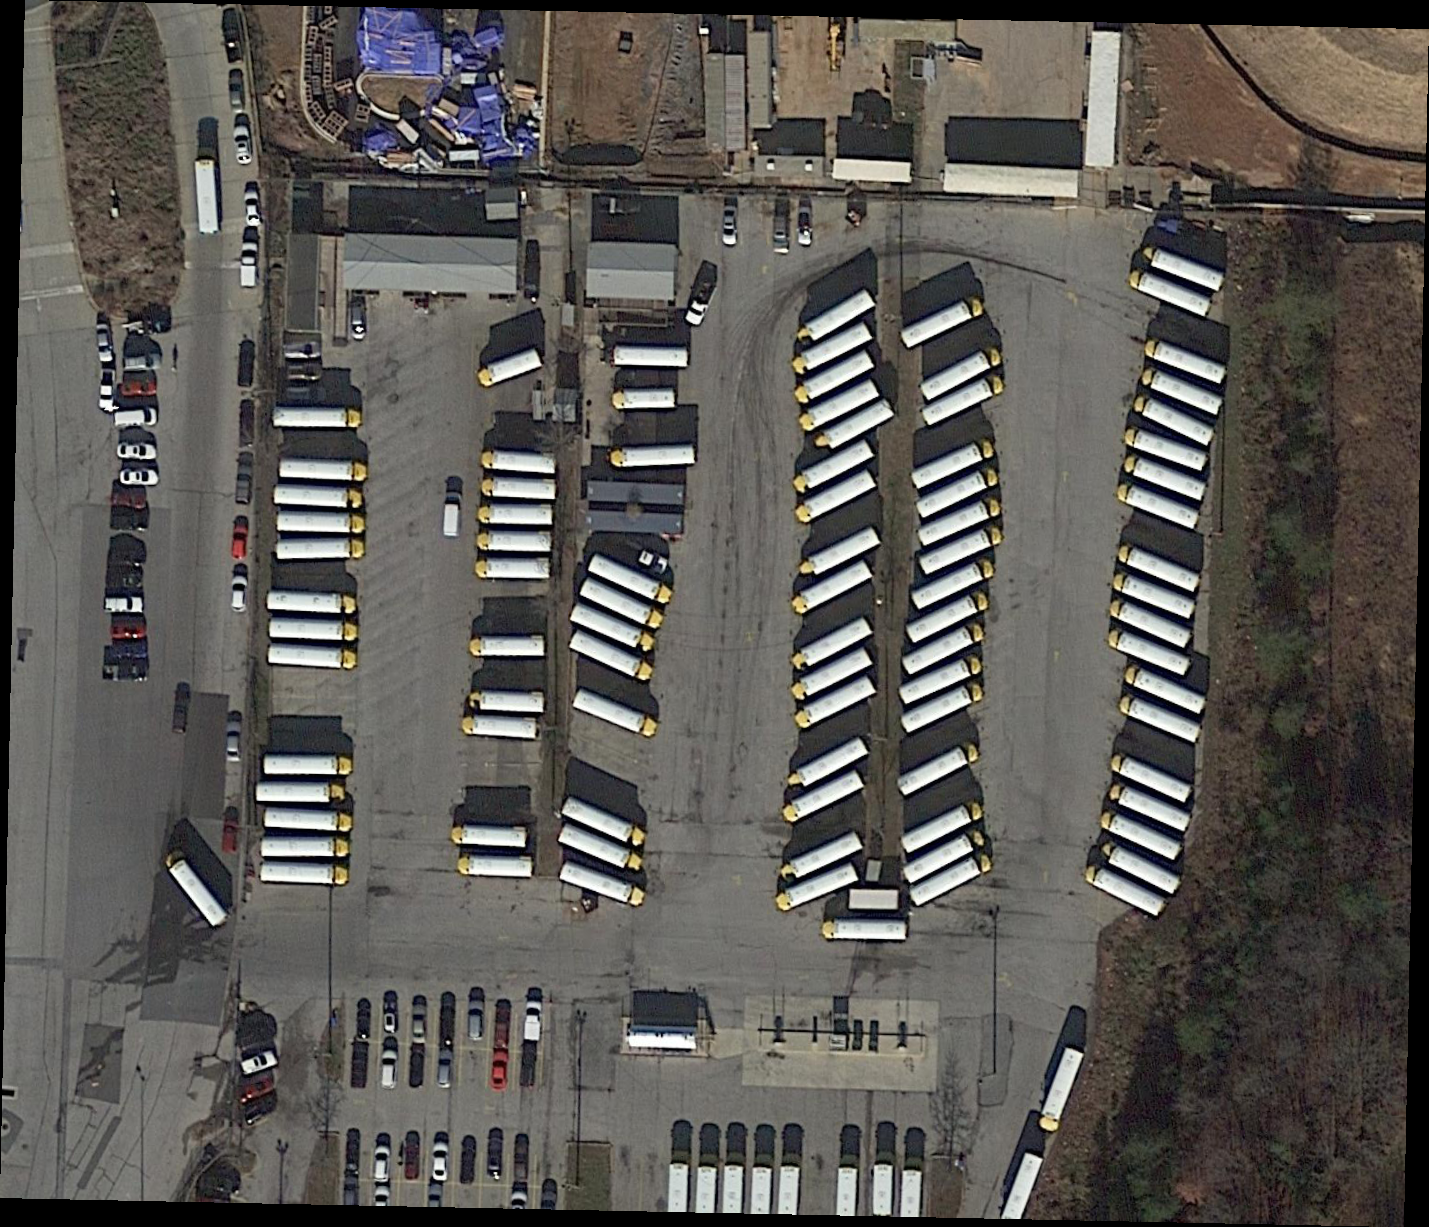
\includegraphics[width=0.45\textwidth]{./Images/isaid.png}
\label{fig:isaid_sample}
}
\hfill
\subfigure[LoveDA Dataset Sample]{
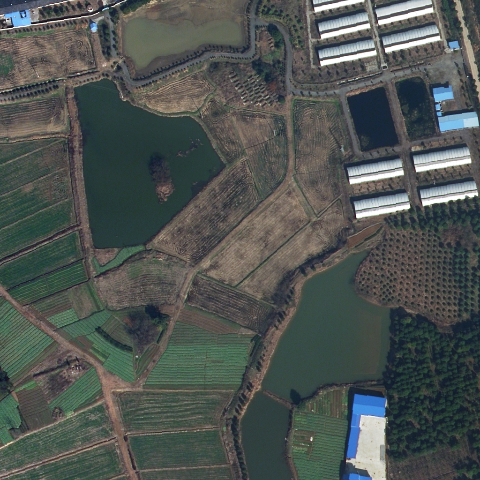
\includegraphics[width=0.45\textwidth]{./Images/loveda.png}
\label{fig:loveda_sample}
}
\caption{Source Dataset Examples}
\label{fig:source_datasets}
\end{figure}

% #############################################################################
\section{Rule-Based Generation Pipeline}

Our rule-based pipeline systematically transforms aerial segmentation datasets into referring expression datasets through spatial analysis, visual feature extraction, and combinatorial expression generation.

\begin{figure}[H]
\centering
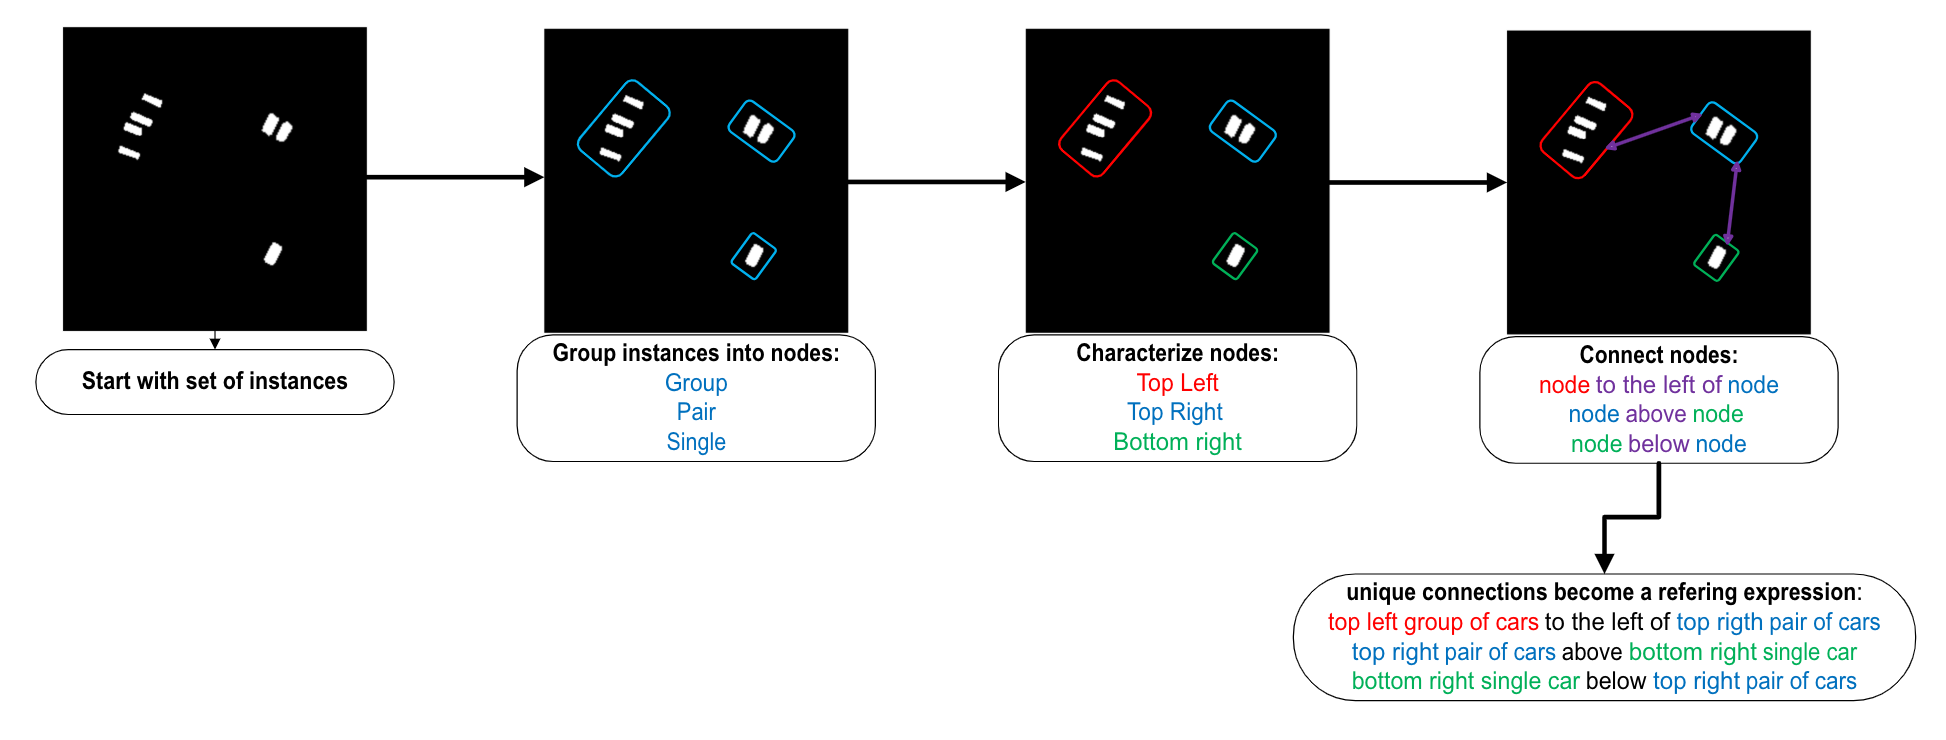
\includegraphics[width=0.8\textwidth]{./Images/rule_based_generation.png}
\caption{Rule-Based Expression Generation Pipeline}
\label{fig:rule_based_pipeline}
\end{figure}

The pipeline consists of multiple sequential steps that analyze spatial relationships, extract visual characteristics, and generate natural language descriptions for aerial objects.

% #############################################################################
\subsection{Expression Filtering and Uniqueness}

After generating the initial set of referring expressions, we apply filtering mechanisms to ensure uniqueness and remove ambiguous descriptions that could refer to multiple objects.

\begin{figure}[H]
\centering
\includegraphics[width=0.8\textwidth]{./Images/filter_unique.png}
\caption{Expression Filtering for Uniqueness}
\label{fig:filter_unique}
\end{figure}

% #############################################################################
\subsection{Generated Expression Examples}

The following figure shows examples of generated referring expressions across different object categories and spatial relationships.

\begin{figure}[H]
\centering
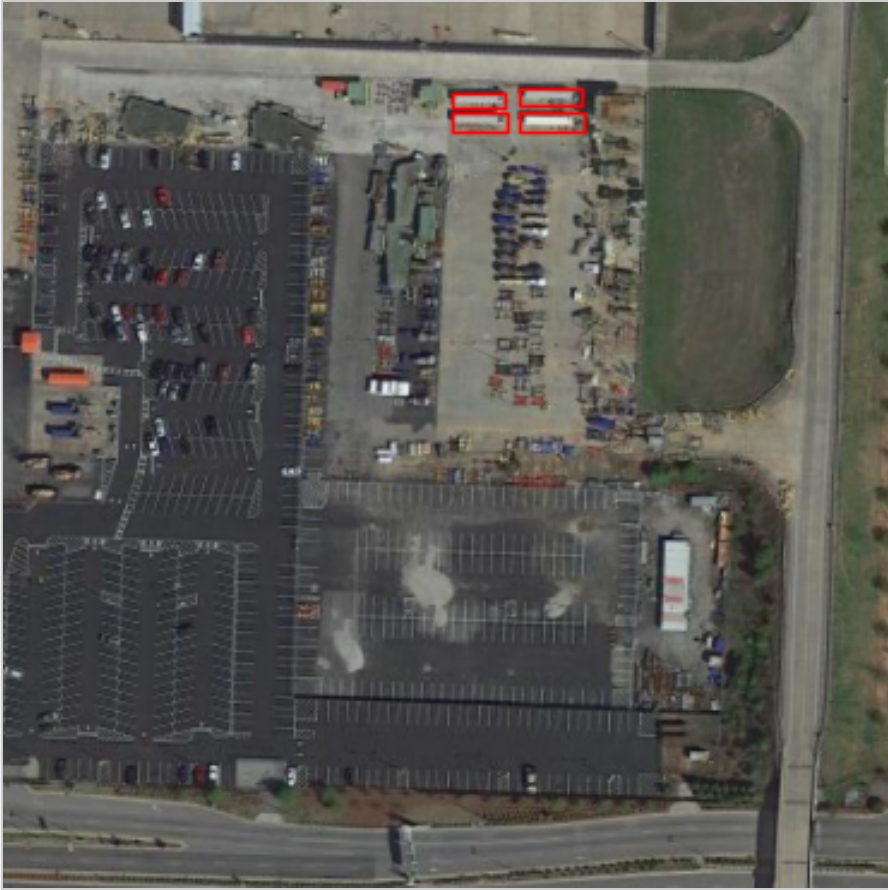
\includegraphics[width=0.9\textwidth]{./Images/example_group.png}
\caption{Examples of Generated Referring Expressions}
\label{fig:expression_examples}
\end{figure}

% #############################################################################
\section{LLM Enhancement Pipeline}

Beyond rule-based generation, we enhance the dataset through multimodal large language model fine-tuning to create more natural and diverse referring expressions.

\begin{figure}[H]
\centering
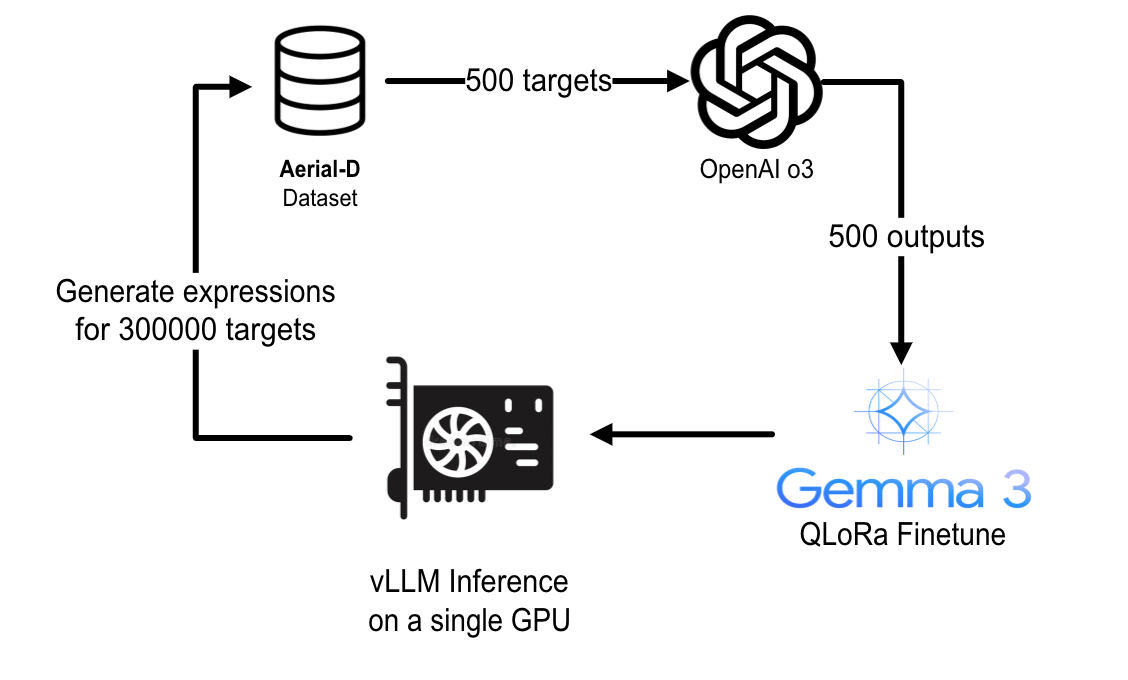
\includegraphics[width=0.8\textwidth]{./Images/distillation.png}
\caption{LLM Enhancement and Knowledge Distillation Pipeline}
\label{fig:llm_distillation}
\end{figure}

% #############################################################################
\section{Dataset Statistics and Composition}
Cras sed ante. Phasellus in massa. Curabitur dolor eros, gravida et, hendrerit ac, cursus non, massa. Aliquam lorem. In hac habitasse platea dictumst. Cras eu mauris \Cref{time_control_algorithm}\todo[color=cyan!40, author=RC, fancyline]{Notice the reference to the Algorithm construct}{}. Quisque lacus. Donec ipsum. Nullam vitae sem at nunc pharetra ultricies. Vivamus elit eros, ullamcorper a, adipiscing sit amet, porttitor ut, nibh. 

\begin{algorithm}[ht]
\DontPrintSemicolon
\Begin{
$nextBitrate \longleftarrow nextDownloadLevel$\;
$nextBitrate \longleftarrow GetNextBitrate()$\;
$cpuLoad \longleftarrow GetCpuLoad()$\;
$bitrateDelta \longleftarrow getBitrateDelta(currentBitrate, nextBitrate)$\;
\BlankLine
\If{$bitrateDelta > maxThreshold$}{
     $SetBitrate(nextBitrate)$\;
   }
\BlankLine
  \If{$minThreshold < bitrateDelta < maxThreshold$ {\bf and} $numAttemps < 2$}{ 
       $numAttemps \longleftarrow numAttemps + 1$\;
       }{
       \uElseIf{$minThreshold < bitrateDelta < maxThreshold$ {\bf and} $numAttemps = 2$}{
       $numAttemps \longleftarrow 0$\;
       }
       \Else{$SetBitrate(nextBitrate)$}
      }
  \If{$0 < bitrateDelta < minThreshold$ {\bf and} $numAttemps < 3$}{
       $numAttemps \longleftarrow numAttemps + 1$\;
       }{
       \uElseIf{$0 < bitrateDelta < minThreshold$ {\bf and} $numAttemps = 3$}{
       $SetBitrate(nextBitrate)$\;
       }
       }
}
\caption{Time Control Strategy}
\label{time_control_algorithm}
\end{algorithm}


Maecenas adipiscing mollis massa. Nunc ut dui eget nulla venenatis aliquet. Sed luctus posuere justo. Cras vehicula varius turpis. Vivamus eros metus, tristique sit amet, molestie dignissim, malesuada et, urna..
% #############################################################################
\section{Client Application}
Cras sed ante. Phasellus in massa. Curabitur dolor eros, gravida et, hendrerit ac, cursus non, massa. Aliquam lorem. In hac habitasse platea dictumst. Cras eu mauris. Quisque lacus. Donec ipsum. Nullam vitae sem at nunc pharetra ultricies. 

Vivamus elit eros, ullamcorper a, adipiscing sit amet, porttitor ut, nibh. Maecenas adipiscing mollis massa. Nunc ut dui eget nulla venenatis aliquet. Sed luctus posuere justo. Cras vehicula varius turpis. Vivamus eros metus, tristique sit amet, molestie dignissim, malesuada et, urna.

Quisque lacus. Donec ipsum. Nullam vitae sem at nunc pharetra ultricies. Cras vehicula varius turpis.



\begin{minipage}[c]{1.0\textwidth}
%\begin{center}
\centering
\begin{lstlisting}[language = C++, numbers = none, escapechar = !,
    basicstyle = \ttfamily\bfseries, linewidth = .6\linewidth, frame=tb, caption={A listing with a Tikz picture overlayed}, captionpos=b, label=tikzlist] 
 int!
   \tikz[remember picture] \node [] (a) {};
 !puissance!
   \tikz[remember picture] \node [] (b) {};
 !(int x,!
   \tikz[remember picture] \node [] (c){};
 !int n) { 

     int i, p = 1; !\tikz[remember picture] \node [] (d){};!           

     for (i = 1; i <= n; i++) 
       p = p * x; !\tikz[remember picture] \node [inner xsep = 40pt] (e){};! 

     return p; !
       \tikz[remember picture] \node [] (f){};!  
 }
\end{lstlisting}

\begin{tikzpicture}[remember picture, overlay,
    every edge/.append style = { ->, thick, >=stealth,
                                  darkgray, dashed, line width = 1pt },
    every node/.append style = { align = center, minimum height = 10pt,
                                 font = \bfseries, fill= green!20},
                  text width = 2.5cm ]
  \node [above left = .75cm and -.75 cm of a,text width = 2.2cm]
                             (A) {return value type};
  \node [right = 0.25cm of A, text width = 1.9cm]
                             (B) {function name};
  \node [right = 0.5cm of B] (C) {list of formal parameters};
  \node [right = 4.cm of d]  (D) {local variables declaration};
  \node [right = 2.cm of e]  (E) {instructions};
  \node [right = 5.cm of f]  (F) {instruction \texttt{\bfseries return}};  
  \draw (A.south) + (0, 0) coordinate(x1) edge (x1|-a.north);
  \draw (B.south) + (0, 0) coordinate(x2) edge (x2|-b.north);
  \draw (C.south) + (0, 0) coordinate(x3) edge (x3|-c.north);
  \draw (D.west) edge (d.east) ;
  \draw (E.west) edge (e.east) ;  
  \draw (F.west) edge (f.east) ;
\end{tikzpicture}
%\end{center}
\end{minipage}

\textcolor{violet}{And here another method (\Cref{tikzlist}) for mixing (overlay) a picture with a listing of code.}
% #############################################################################
\subsection{User Interface}
Donec semper turpis sed diam. Sed consequat ligula nec tortor. Integer eget sem. Ut vitae enim eu est vehicula gravida. Morbi ipsum ipsum, porta nec, tempor id, auctor vitae, purus. Pellentesque neque. Nulla luctus erat vitae libero. Integer nec enim. Phasellus aliquam enim et tortor. Quisque aliquet, quam elementum condimentum feugiat, tellus odio consectetuer wisi, vel nonummy sem neque in elit. Curabitur eleifend wisi iaculis ipsum. Pellentesque habitant morbi tristique senectus et netus et malesuada fames ac turpis egestas. In non velit non ligula laoreet ultrices. Praesent ultricies facilisis nisl. Vivamus luctus elit sit amet mi. Phasellus pellentesque, erat eget elementum volutpat, dolor nisl porta neque, vitae sodales ipsum nibh in ligula. Maecenas mattis pulvinar diam. Curabitur sed leo..

Cras eu mauris. Quisque lacus. Donec ipsum. Nullam vitae sem at nunc pharetra ultricies. Vivamus elit eros, ullamcorper a, adipiscing sit amet, porttitor ut, nibh. Maecenas adipiscing mollis massa. Nunc ut dui eget nulla venenatis aliquet. Sed luctus posuere justo. Cras vehicula varius turpis. 
% #############################################################################
\subsection{Vivamus luctus elit sit amet mi}
Nulla facilisi. In vel sem. Morbi id urna in diam dignissim feugiat. Proin molestie tortor eu velit. Aliquam erat volutpat. Nullam ultrices, diam tempus vulputate egestas, eros pede varius leo, sed imperdiet lectus est ornare odio. Lorem ipsum dolor sit amet, consectetuer adipiscing elit. Proin consectetuer velit in dui. Phasellus wisi purus, interdum vitae, rutrum accumsan, viverra in, velit. Sed enim risus, congue non, tristique in, commodo eu, metus. Aenean tortor mi, imperdiet id, gravida eu, posuere eu, felis. 

Mauris sollicitudin, turpis in hendrerit sodales, lectus ipsum pellentesque ligula, sit amet scelerisque urna nibh ut arcu. Aliquam in lacus. 

\Cref{fig:ui_playout,fig:ui_loading}\todo[color=cyan!40, author=RC, fancyline]{A figure with Subfigures}{} proin at eros non eros adipiscing mollis.

\begin{figure}[htbp]
	\centering
	\subfigure[Media Loading Window]{\label{fig:ui_loading} 		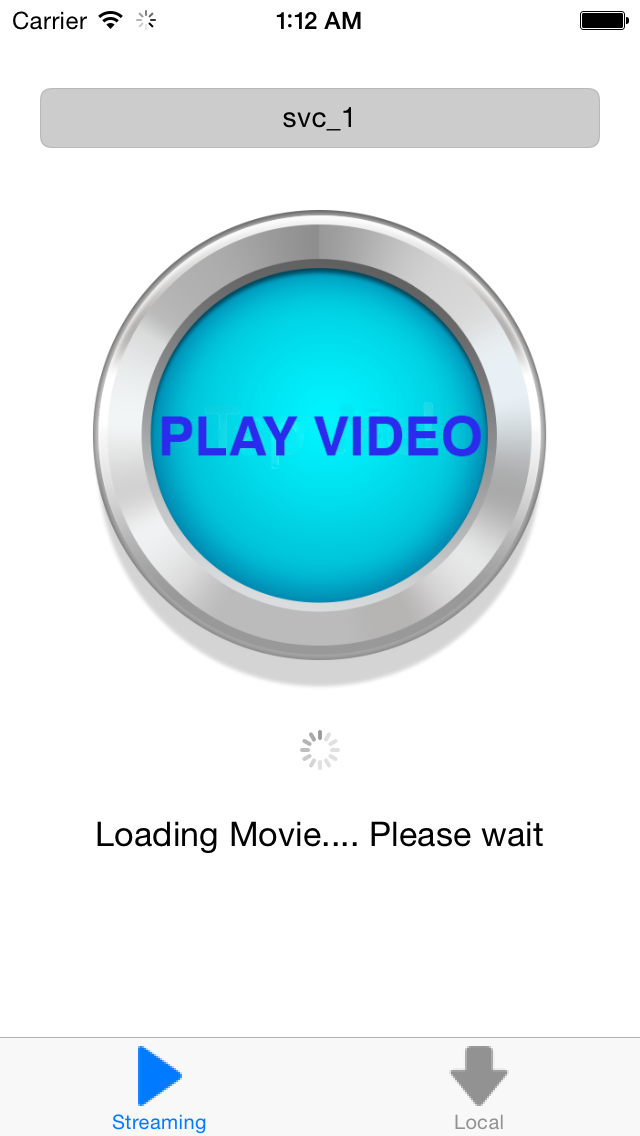
\includegraphics[width=0.3\textwidth]{./Images/ui_loading}} \qquad
	\subfigure[Play-out Session UI]{\label{fig:ui_playout}
		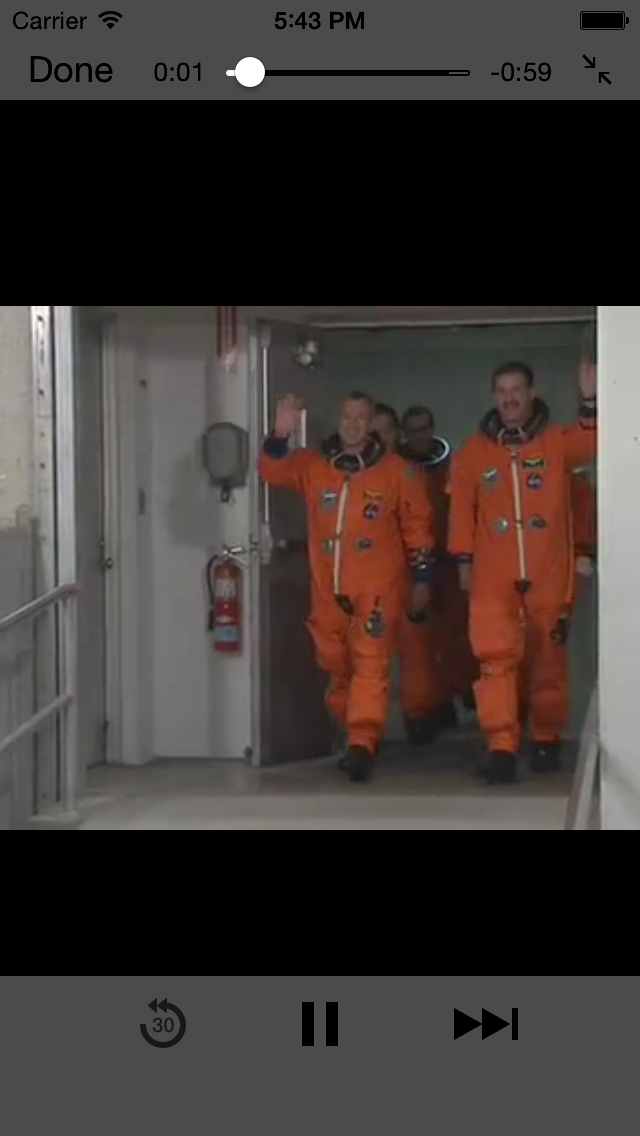
\includegraphics[width=0.3\textwidth]{./Images/ui_playout}}
	\caption{Complete User Interface}
	\label{fig:user_interface}
\end{figure}

Vestibulum ante ipsum primis in \ac{UI} faucibus orci luctus et ultrices posuere cubilia Curae; Nulla placerat aliquam wisi. Mauris viverra odio. Quisque fermentum pulvinar odio. Proin posuere est vitae ligula. Etiam euismod. Cras a eros.